\documentclass{article}

\usepackage{amsmath, amsthm, bm, physics, enumerate, siunitx, dirtytalk, tikz}
\usepackage{hyperref}
\usetikzlibrary{calc, patterns}

\newtheorem{theorem}{Theorem}
% \newtheorem{lemma}{Lemma}

% \providecommand{\levicivita}[3]{%
%   \ensuremath{\varepsilon_{{#1}{#2}{#3}}}
% }


% ------------------------------------------------------------------------------
\title{Derivation of momentum conservation law\\
\large \textit{based on the lecture of prof.\ Andrzej Styczek}}
\author{Wojciech Sadowski}

\begin{document}
\maketitle

\section{Basics}

\paragraph{What is a fluid?}
We will consider a fluid as a continuous substance. That is, the fluid fills
fully available space. Therefore, \emph{we are neglecting the discrete nature
of matter.} We can do that, since the amount of fluid molecules in small volume 
of matter is gargantuan (remember the Avogadro number \(N_a\approx\SI{6.023e26}{kmol^{-1}}\)).

It is painfully difficult to describe the motion of each and every molecule 
constituting the fluid. Apart from the obvious problem of integrating all of 
the trajectories we also encounter a problem of determining an accurate initial
conditions for every molecule. In such systems, a small error in determining 
these starting parameters will unfortunately lead to considerable inaccuracies
further down the line.

Hence, we neglect the discrete nature of matter. The medium, i.e.\ fluid, consists 
of continuous set of ideal particles\footnote{%
A point that might have mass or charge or some other 
property. From Wikipedia: \say{an idealization of particles 
[...]. Its defining feature is that it lacks spatial extension; being dimensionless,
it does not take up space.}}.
So the movement of the medium is 
\emph{de facto} the movement of the points, and such description can be 
used for solids (a continuous medium retaining some shape or natural configuration),
fluids and \say{things} in between. Fluids do not have this natural, reference 
configuration: the relative positions of the points can be arbitrary and changing.
Sometimes we might assume that volume of fluid has to be conserved (or that the 
density is constant) but that is, of coarse, a simplification. A useful and 
accurate one in situations of non-varying thermodynamic state of the medium.

If this \say{reference shape} does not exist, than the deformation (or strain) of the fluid
can be completely arbitrary. \emph{Water spilled on the floor will deform greatly,
covering the area and seeping into the cracks, potentially making you call the 
handyman to fix the broken flooring.} So what creates the internal forces inside 
the fluid? One obvious answer is the change of volume, but what else?

We will consider fluids in which the forces depends on the rate of deformation. 
These forces clearly will \say{want} to stop, or counteract, the deformation 
occurring in the fluid. As we have already discussed, the deformation itself 
does not seem to be important.

However, it is important to indicate, that this is only a simplified model, 
not existing in nature. In the same way as each fluid is really compressible,
this assumption is a useful lie. For  
the most general fluid we could write
\[
  f(t, \bm{\tau}, \dot{\bm{\tau}}, \bm{D}, \dot{\bm{D}}, \dots) = 0,
\]
and call it \emph{constitutive equation}, i.e.\ a relation defining our material.
It describes connection between the time \(t\), stresses \(\bm{\tau}\), deformation \(\bm{D}\),
the rates of those things (indicated by the same letters with a dot accent) 
and potentially other parameters.

As you can see, it can be bad. The parameters in the above relations could
depend on each other or they could depend on each other non-locally (i.e.\ point
\(a\) depends on the state in point \(b\)). Or even worse, they might be influenced
by the history of the those parameters. Fortunately, for most of classical use 
cases we can confine ourselves to much simpler relations.

We will say:
\begin{enumerate}[(i)]
  \item only \(\bm{\tau}\) and \(\dot{\bm{D}}\) are important;
  \item the relation between them is defined in the same place and time;
  \item we should be able two solve for \(\bm{\tau}\), that is write
    \(
      \bm{\tau} = g(\dot{\bm{D}});
    \)
  \item the relationship should not have any preferential direction, that 
    is, for example, the fluid should not behave differently along the \(x\) 
    or \(y\) axis (in practice, this will require that the \(\bm{\tau}\) and
    \(\dot{\bm{D}}\) are \emph{symmetric}). 
\end{enumerate}

\paragraph{What are stresses?}
We know what a \emph{force} is. Intuitively,
when thinking about fluids or materials, the stress is a force acting on 
a surface. We also know that we can add forces, so we can safely assume that
the sum of forces acting on parts of the surface have to add up to the force 
acting on the whole surface. Let's define force differential \(\dd{\vb{F}}\) acting 
on a small part of the surface \(\dd S\), in a following way
\[
  \dd \vb{F} = \vb{f}\dd{S},
\]
so that \(\vb{f}\) becomes a force per unit surface, so surface force density.

Let us consider a Cartesian coordinate system \((O, x_1, x_2, x_3)\) and 
a small tetrahedron with walls \(\dd S_1\), \(\dd S_2\), \(\dd S_3\) and 
closed by the wall \(\dd S\) (see \autoref{fig::force_tetrahedron}). There 
can be infinite amount of such tetrahedrons, however the numbered walls 
\(\dd S_i\) are always laying on the same planes, perpendicular to the 
axis of the system. On the other hand, wall \(\dd S\) changes its position
along with the plane its laying on and the surface area. 

\begin{figure}[bh!]
  \centering
  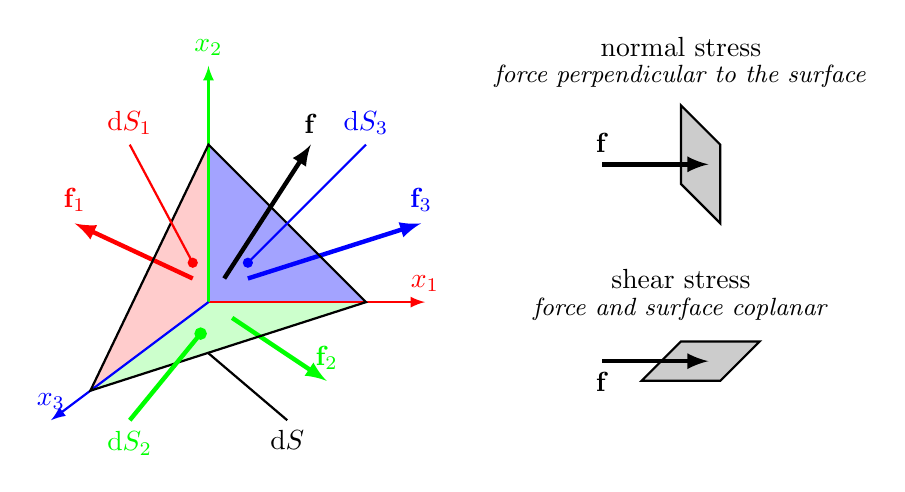
\begin{tikzpicture} 
    \fill [red, fill opacity = 0.2] (0cm, 0cm) -- (-2cm * 0.75, -1.5cm * 0.75) -- (0cm, 2cm) -- cycle;
    \fill [green, fill opacity = 0.2] (0cm, 0cm) -- (-2cm * 0.75, -1.5cm * 0.75) -- (2cm, 0cm) -- cycle;
    \fill [blue, fill opacity = 0.2] (0cm, 0cm) -- (2cm, 0cm) -- (0cm, 2cm) -- cycle;
    \fill [blue, fill opacity = 0.2] (0cm, 0cm) -- (2cm, 0cm) -- (0cm, 2cm) -- cycle;
 
    \draw [red, -latex, ultra thick] 
    (-0.2cm, 0.3cm) -- (-1.7cm, 1cm) node [above] {$\vb{f}_1$}; 
    \draw [blue, -latex, ultra thick] 
    (0.5cm, 0.3cm) -- (2.7cm, 1cm) node [above] {$\vb{f}_3$}; 
    \draw [green, -latex, ultra thick] 
    (0.3cm, -0.2cm) -- (1.5cm, -1cm) node [above] {$\vb{f}_2$}; 

    \draw [-latex, thick, red] (0cm, 0cm) -- (2.75cm, 0cm) node [above] {$x_1$};
    \draw [-latex, thick, green] (0cm, 0cm) -- (0cm, 3cm) node [above] {$x_2$};
    \draw [-latex, thick, blue] (0cm, 0cm) -- (-2cm, -1.5cm) node [above] {$x_3$};
    \draw [thick] (-2cm * 0.75, -1.5cm * 0.75)  -- (2cm, 0cm) -- (0cm, 2cm) -- cycle;
    % \fill [pattern=north west lines, pattern color=black] (-2cm * 0.75, -1.5cm * 0.75)  -- (2cm, 0cm) -- (0cm, 2cm) -- cycle;
    
    \draw [blue, thick] (0.5cm, 0.5cm) -- (2cm, 2cm)
      node [pos=1, above] {$\dd S_3$}  
      node [draw=blue, circle, fill=blue, inner sep=1pt, pos=0]  {}; 
    \draw [red, thick] (-0.2cm, 0.5cm) -- (-1cm, 2cm)
      node [pos=1, above] {$\dd S_1$}  
      node [draw=red, circle, fill=red, inner sep=1pt, pos=0]  {}; 
    \draw [green, ultra thick] (-0.1cm, -0.4cm) -- (-1cm, -1.5cm)
      node [pos=1, below] {$\dd S_2$}  
      node [draw=green, circle, fill=green, inner sep=1pt, pos=0]  {}; 
    \draw [black, thick] (0cm, -0.65cm) -- (1cm, -1.5cm)
      node [pos=1, below] {$\dd S$};

    \draw [ultra thick, -latex] (0.2cm, 0.3cm) -- (1.3cm, 2cm) 
      node [above] {$\vb{f}$};

    % \node at (4cm, 3cm) [anchor = north west] {%
    %   \parbox{4cm}{%
    %   Equilibrium condition:\\
    %   \(\vb{f}_i \dd S_i+ \vb{f}\dd S =\vb{0}\)
    %   }};
    \begin{scope}[xshift=1cm]
    \draw [fill, color = black, fill opacity=0.2, thick] 
      (5cm, 2.5cm) -- (5.5cm, 2cm) 
      -- (5.5cm, 1cm) -- (5cm, 1.5cm) -- cycle ;
    \node at (5cm, 3cm) [above] {normal stress};
    \node at (5cm, 2.60cm) [above] 
    {\small \textit{force perpendicular to the surface}};
  
    \draw [-latex, ultra thick] (4cm, 1.75cm) -- (5.35cm, 1.75cm)
      node [above, pos=0] {$\vb{f}$};

    \node at (5cm, 0.05cm) [above] {shear stress};
    \node at (5cm, -0.35cm) [above] 
    {\small \textit{force and surface coplanar}};
    \draw [fill, color = black, fill opacity=0.2, thick]
      (5cm, -0.5cm) -- (6cm, -0.5cm) -- (5.5cm, -1cm) 
      -- (4.5cm, -1cm) -- cycle;
    \draw [-latex, ultra thick] (4cm, -0.75cm) -- (5.35cm, -0.75cm)
      node [below, pos=0] {$\vb{f}$};
    \end{scope}
  \end{tikzpicture}
  \caption{Elementary tetrahedron}
  \label{fig::force_tetrahedron}
\end{figure}

If this volume is in equilibrium, than the forces acting on the walls, 
\(\vb{f}_1\), \(\vb{f}_2\), \(\vb{f}_3\) and \(\vb{f}\) respectively,
add up to \(\vb{0}\)
\begin{equation}\label{eq::equilibrium}
  \vb{f}_1 \dd{S_1} 
  + \vb{f}_2 \dd{S_2} 
  + \vb{f}_3 \dd{S_3} 
  + \vb{f} \dd{S} = \vb{f}_i \dd{S_i} + \vb{f} \dd{S} = \vb{0}.
\end{equation}
Let us divide the equation by \(\dd{S}\)
\[
  \vb{f}_i \dfrac{\dd{S_i}}{\dd{S}} + \vb{f} = \vb{0}.
\]
We do that because we notice that the fraction \(\dd{S} / \dd{S_i}\) is
equal to the cosine of the angle between the normal of \(\dd{S}\) and 
the \(i\)-th axis of the coordinate system (believe me, or prove it 
if you don't). We can also say that \(\cos(\bm{n}, x_i) = n_i\) and we will
use that later. 

In \autoref{eq::equilibrium} we didn't assume anything about the directions
of the forces, however, if the tetrahedron is in equilibrium, than the sum of 
\(\vb{f}_i\) has to be opposite to \(\vb{f}\). Hence, we can flip it noting
that if we change direction, the sign changes as well, i.e.\ 
\(\vb{f}(\vb{n}) = -\vb{f}(-\vb{n})\). 
After substituting our \say{revolutionary} findings about the 
\(\dd{S} / \dd{S_i}\) ratio equal to the cosine as well, we are left with the following relation
\[
  \vb{f} = \vb{f}_i \dfrac{\dd{S_i}}{\dd{S}} 
  = \vb{f}_i\cos(\bm{n}, x_i) 
  = \vb{f}_i n_i  
\]

Now, considering that each force has three components, which for example for 
\(\vb{f}_1\) we will denote as \(f_{11}\), \(f_{12}\) and \(f_{13}\), we can 
also write the equation for \(k\)-th component of \(\vb{f}\)
\[
  f_k = n_1 f_{1k} + n_2 f_{2k} +n_3 f_{3k} = n_\alpha f_{\alpha k}.
\]
So, we actually have arrived at something! We have \emph{nine} numbers giving
together the components of \(f_{\alpha k}\), which describe the forces acting 
on the surface closing our small tetrahedron. Furthermore, if you shrink the 
tetrahedron to a point (we already used differentials of surfaces), what we 
wrote above still holds! This means that, the force density acting on a surface 
in the fluid depends on those nine numbers and the orientation of the surface.

We will call those numbers stresses. Make a though experiment: imagine a force 
acting in a chosen direction, and a surface perpendicular to this force. This 
is aligned with the classical definition of pressure, right? Now, rotate this 
surface, so that the force vector lies on the surface. Force acting along the 
surface can be understood as shear. That's how scissors work! Now, rotate the 
surface keeping the normal as an axis. The force is now \say{shearing} the 
surface in a different direction, so for one force vector we can have one normal 
(perpendicular to the surface)
stress and we observed two shear stresses. With that (hopefully) intuitive 
explanation we can say that among the nine numbers, we will have \emph{three}
normal stress components and \emph{six} components related to shear stress.

The only problem is the fact that our notation is cumbersome; we have two \(f\)
symbols. Let's set the magic nine numbers (they will get a name soon, I promise!) 
as \(\tau_{ij}\), giving us:
\[
  f_i = n_\alpha \tau_{\alpha i}
\]

\paragraph{Stress tensor}
Okay, so as I said, the nine-number-thingy needs a name. You saw the paragraph
title, you might already now what it is. That said, this is written in style of 
a lecture, so please make a dramatic pause in your brain before reading the end of the 
next sentence. We will call \(\tau_{ij}\) the \emph{stress tensor}. 

But what is a tensor, you might ask? My colleague said at some point\footnote{In Dresden, on the 1st of June, during breakfast, around 9:30 PM.} that a tensor
is just a \say{glorified vector}. This is not really true, but it is a useful starting point for a discussion. 
In fact, some vectors 
\emph{are} tensors. Generally, a tensor is a \say{geometrical thing}, that is,
it describes some effect independent on the coordinate system. Velocity vector
is a tensor or order 1, as it describes that an object moves in a specific direction 
with a specific velocity\footnote{Not every vector is a tensor, e.g.\ the vector
position vector is always dependant on the chosen coordinate system.}. If we
change the basis (coordinate system), the representation, that is the components 
of the vector will change, but the vector itself still points in the same 
direction. \emph{It is a geometric concept.} Similarly to our velocity example, 
stress tensor also describe a distribution of forces inside the material. In 
nature there are no principal, favoured directions, so the object describing it 
should be a tensor.

So, there is some geometric transformation
that tells us how to change the components of a tensors, and tensors 
are objects that obey this transformation. 
This paraphrase of a mathematical mathematical definition is
frankly quite unhelpful\footnote{% 
For interested here is slightly paraphrased version of a definition, 
again stolen from Wikipedia: A tensor of type \((p,q)\) is an assignment 
of a multidimensional array
\[
  T^{i_1\dots i_p}_{j_{1}\dots j_{q}}[\mathbf{f}]
\]
to each basis \(\vb{f} = (\vb{e}_1, \dots, \vb{e}_n)\) of an \(n\)-dimensional 
vector space such that, if we apply the change of basis
\[
  \mathbf{f}\mapsto \mathbf{f}\cdot R = \left( \mathbf{e}_i R^i_1, \dots, \mathbf{e}_i R^i_n \right)
\]
then the multidimensional array obeys the transformation law
\[
  T^{i'_1\dots i'_p}_{j'_1\dots j'_q}[\mathbf{f} \cdot R] = \left(R^{-1}\right)^{i'_1}_{i_1} \cdots \left(R^{-1}\right)^{i'_p}_{i_p}
  T^{i_1, \ldots, i_p}_{j_1, \ldots, j_q}[\mathbf{f}]
  R^{j_1}_{j'_1}\cdots R^{j_q}_{j'_q} .
\]
}.
So we will cheat a little 
and describe a tensor with as much verbosity as is necessary for our use case.

Let's define some operations first and show them on the example of the stress 
tensor, which we will represent here as
\[
  \bm{\tau} = \tau_{ij}\hat{\vb{e}}_i \hat{\vb{e}}_j.
\]
We used the versors \(\hat{\vb{e}}_i\) defining our chosen coordinate system. 
They are multiplied in a weird way, its neither scalar nor vector product. This 
operation is also sometimes written with 
the \(\otimes\) symbol (\(\hat{\vb{e}}_i \otimes \hat{\vb{e}}_j\)) and 
is called tensor or outer product.

The scalar product \(\vb{n}\dotproduct\bm{\tau}\) can be written easily 
with index notation. We know that \(\vb{n} = n_k \hat{\vb{e}}_k\), so 
building on that we can write
\[
  \vb{n}\dotproduct\bm{\tau} 
  = n_k \hat{\vb{e}}_k \dotproduct \qty(\tau_{ij}\hat{\vb{e}}_i \hat{\vb{e}}_j)
  = n_k \tau_{ij} \hat{\vb{e}}_k \dotproduct \hat{\vb{e}}_i \hat{\vb{e}}_j 
  = n_k \tau_{ij} \qty(\hat{\vb{e}}_k \dotproduct \hat{\vb{e}}_i) \hat{\vb{e}}_j.
\]
We can think a little about the term \(\hat{\vb{e}}_k \dotproduct \hat{\vb{e}}_i\).
It is a dot product of two versors. It can be either equal to 1 if they are 
the same (\(k=i\)) or 0 if they are different. There is a term for that, called
\emph{Kronecker delta}, defined as
\[
  \delta_{ij} = \begin{cases}
0 &\text{if } i \neq j,   \\
1 &\text{if } i=j.   \end{cases}
\]
So we can write that our product is equal to 
\(n_k \tau_{ij}\delta_{ki} \hat{\vb{e}}_j \). It does not help us yet, but if 
we said that \(k\) has to be equal to \(i\), otherwise the terms in the sum 
will be 0, we might as well write \(i\) instead of \(k\)\footnote{If you are 
confused try it out on paper, write every term, eliminate the ones equal to 0
and collapse the term to the indexed expression.}, i.e.\
\[
  \vb{n}\dotproduct\bm{\tau} = n_i \tau_{ij} \hat{\vb{e}}_j = f_j \hat{\vb{e}}_j.
\]
In the above, we eliminated \(\delta_{ii}\) as it is always equal to 1. In fact,
\(\delta_{ij}\) is sometimes called an \say{index renamer} as it renames index 
\(j\) to \(i\) or \textit{vice versa}.

Okay, so what have we learned? The dot product of a tensor with a vector gives 
us a vector. Will multiplication from the left, which we performed above, be 
different from the one from the right, that is \(\bm{\tau}\dotproduct\vb{n}\)?
Yes\footnote{I am to lazy to write it down, but it might be a good training
for you.}. That said, it would be the same if \(\tau_{ij} = \tau_{ji}\).

So a lot of hints have been dropped. The tensor behaves a little bit like a 
matrix. In fact the matrix is often used to \emph{represent} a tensor in a 
chosen coordinate system, but the tensor itself, like a velocity vector, is 
independent from the chosen coordinate system\footnote{Stress tensor has rank 2; we 
used two versors, so called diad, to define it.}. This matrix can be multiplied with a vector to give 
another vector. If the matrix is symmetric, product from both sides will return vectors 
with the same components. Kronecker delta is also a tensor itself, represented by
a unit matrix \(\bm{I}\).

\paragraph{Strain-rate (deformation-rate) tensor}
It was mentioned, that we are interested in a tensor defining a rate of 
deformation, or what is usually called \emph{strain-rate tensor} in 
literature. We should derive it. Let's start with a series expansion of 
velocity field around coordinate \(\vb{r}\):
\[
  v_i(t, \vb{r} + \dd{\vb{x}}) = v_i(t, \vb{r}) + \pdv{v_i}{x_k}\dd{x_k}
  + \dots
\]
If \(\dd{x}\rightarrow\vb{0}\), we disregard the higher order terms and 
rewrite the above as 
\[
  v_i(t, \vb{r} + \dd{\vb{x}}) = v_i(t, \vb{r}) 
  + \frac{1}{2}\qty(\pdv{v_i}{x_k} + \pdv{v_k}{x_i})\dd{x_k}
  + \frac{1}{2}\qty(\pdv{v_i}{x_k} - \pdv{v_k}{x_i})\dd{x_k}.
\]
The first term on the right describes simple translation of the fluid parcel.
The third (similar to the expression for the curl of velocity field) defines
rotation. Both of these can be applied to the rigid, unchanging in shape, 
fluid parcel. We are left with the second one, describing the change of 
velocity due to \say{non-rigid} strain or deformation of the fluid volume. 
We can write this change of velocity mathematically as
\begin{equation}\label{eq::strain_rate_tensor}
  \dd{v^\mathrm{strain}_k} 
  = \frac{1}{2}\qty(\pdv{v_i}{x_k} + \pdv{v_k}{x_i})\dd{x_k}
  = \dot{D}_{ik}\dd{x_k}
\end{equation}
The tensor \(\dot{\vb{D}}\) is the strain-rate tensor and very importantly 
it is \emph{symmetric}!

\section{Momentum equation I: General form}

\section{Fluid constitutive relations}

We should now try to derive the formulas for \(\bm{\tau}\) so we can plug
them into the momentum equation, be done with this derivation and go home.
Let's start with a simple model of an \emph{inviscid} fluid. If the fluid
has no viscosity, than pressure should be the only thing contributing to 
the stress tensor. \emph{For the sake of later discussion, please note that 
this is the same situation as in the non-moving viscous fluid.} We remember
Pascal's law
\begin{quote}
  \say{Any two points at the same elevation in a continuous mass of the same 
  static fluid will be at the same pressure}\footnote{%
  White, F.M. (2016) Fluid mechanics. Eighth edition. New York, 
  NY: McGraw-Hill Education.}
\end{quote}
here stated assuming hydrostatic distribution of pressure. If we don't have 
any favoured direction it can be rephrased as
\begin{quote}
  \say{The pressure applied to any part of the enclosed liquid will be 
  transmitted equally in all directions through the liquid}\footnote{%
    Wikipedia (Accessed 01.06.2023), Pascal's law}
\end{quote}
We can than represent the force density acting at \(\dd{S}\) as 
\[
  \vb{f} = -\vb{n}p,
\]
where \(p\) represents pressure. We assume that the normal vector \(\vb{n}\) is
directed outside of a fluid parcel that we are considering. The minus in front 
of the expression, is there due to the fact that the surface exerts the pressure
inwards. If we note that \(\vb{f} = \vb{n}\dotproduct\bm{\tau}\) we can now say
\[
  \vb{f} = \vb{n}\dotproduct\bm{\tau} = -\vb{n}p = \vb{n}\dotproduct \qty( -p\vb{I} ) 
  \rightarrow \bm{\tau} = -p \vb{I}
\]
or in the index notation \(\tau_{ij} = -p \delta_{ij}\).

\paragraph{Including strain-rate}
Let's generalise. As we mentioned before, we are looking for 
relation of the form \(\bm{\tau} = g(\dot{\vb{D}})\). We would like to do the
power expansion of \(g\)\footnote{Power series around 0 looks like that: 
\(k(x) = k(0) + ax + bx^2 + \dots\)}. We will have a constant part (independent 
of the function argument), linear, quadratic and so on. In our case, the 
constant part can be conveniently expressed as
\(g(\dot{\vb{D}})_{\dot{\vb{D}} = \vb{0}}\). This situation is exactly like the 
one before, we have no deformation, so the fluid is probably not moving. So
we can write:
\[
  \bm{\tau} = -p\vb{I} + \text{linear term w.r.t. } \dot{\vb{D}} 
                       + \text{quadratic term w.r.t. } \dot{\vb{D}} + \dots
\]
We have the constant term and now we need to determine the other ones.

\paragraph{Eigenvalue problem for a tensor}
For every tensor, it can \say{act} on a vector to produce another vector, as 
in \(M_{\alpha\beta}a_\beta = b_\alpha\) or \(\vb{M}\vb{a} = \vb{b}\). If we 
have selected a special vector \(\vb{a}\), the resultant vector \(\vb{b}\)
might be collinear with \(\vb{a}\). This property is a geometric fact, 
independent of the chosen coordinate system. So if we set this special
vector as \(\vb{q}\) and following is true
\[
  \vb{M}\vb{q} = \lambda\vb{q} \quad \text{or} \quad 
  \qty(\vb{M} - \lambda\vb{I})\vb{q} = \vb{0},
\]
than both \(\lambda\), called an \emph{eigenvalue}, and \(\vb{q}\), the 
\emph{eigenvector} do not depend on the coordinate system.
For \(\vb{q}\) not to be a trivial \(\vb{0}\), following determinant has to 
vanish
\[
  \det(\vb{M} - \lambda\vb{I}) = 0.
\]
If we actually spell the determinant out we will get the third order 
equation for \(\lambda\):
\begin{equation}\label{eq::characterstic_equation}
  -\lambda^3 + I_1 \qty(\vb{M})\lambda^2 - I_2\qty(\vb{M})\lambda 
  + I_3\qty(\vb{M}) = 0.
\end{equation}
It is called \emph{characteristic equation} of a tensor (or a matrix). The 
scalars \(I_1\), \(I_2\) and \(I_3\) depend on \(\vb{M}\). We established 
that eigenvectors do not depend on the coordinate system, they \say{zero}
\autoref{eq::characterstic_equation}, so the coefficients of the equation,
that is \(I_1\), \(I_2\) and \(I_3\), also have to be independent from the 
chosen system. They are called \emph{invariants} and are given by the 
following relations\footnote{Shamelessly stolen from Wikipedia (accessed 
01.06.2023), Invariants of tensors}:
\begin{align*}
  I_1 &= \mathrm{tr}(\mathbf{M}) = M_{11}+M_{22}+M_{33} = \lambda_1+\lambda_2+\lambda_3 \\ 
  I_2 &= \frac{1}{2} \left( (\mathrm{tr}(\mathbf{M}))^2-\mathrm{tr} \left( \mathbf{M}^2 \right) \right) \\
      &= M_{11}M_{22}+M_{22}M_{33}+M_{11}M_{33}-M_{12}M_{21}-M_{23}M_{32}-M_{13}M_{31} \\
      &= \lambda_1 \lambda_2 + \lambda_1 \lambda_3 + \lambda_2 \lambda_3 \\
  I_3 &= \det (\mathbf{M}) = -M_{13} M_{22} M_{31} + M_{12} M_{23} M_{31} + M_{13} M_{21} M_{32} \\
      &- M_{11} M_{23} M_{32} - M_{12} M_{21} M_{33} +   M_{11} M_{22} M_{33} = \lambda_1 \lambda_2 \lambda_3
\end{align*}
Naturally, remembering those formulas is not useful, but it is good to 
remember that they exist. We will now introduce a theorem that will do 
a lot of work for us.
\begin{theorem}[Cayleya–Hamilton theorem]
   Every square matrix over a commutative ring (such as the real or 
   complex numbers or the integers) satisfies its own characteristic equation.
\end{theorem}
\noindent
In practice, this means that the following holds
\begin{equation*}
  -\vb{M}^3 + I_1 \qty(\vb{M})\vb{M}^2 - I_2\qty(\vb{M})\vb{M}
  + I_3\qty(\vb{M})\vb{I} = 0.
\end{equation*}
We essentially substituted \(\vb{M}\) into \autoref{eq::characterstic_equation}.
What can now rearrange and obtain closed expression for \(\vb{M}^3\)
\begin{equation}\label{eq::third_power}
  \vb{M}^3  = - I_1 \qty(\vb{M})\vb{M}^2 + I_2\qty(\vb{M})\vb{M}
  - I_3\qty(\vb{M})\vb{I}
\end{equation}
and \(\vb{M}^4\) and so on.

\paragraph{Constitutive relation: coefficient of the power series}
So from what we have said before, we can say that all powers of the 
series describing \(\bm{\tau} = g(\dot{\vb{D}})\) above the second one
are not linearly independent from each other. So we can safely limit the 
expansion to first two and another constant term. W can write
\[
  \bm{\tau} = -p\vb{I} + \gamma_1 \vb{\dot{D}} + \gamma_2\vb{I} 
  + \gamma_3\vb{\dot{D}}\vb{\dot{D}}
\]
Couple of things happened here. First we substituted \autoref{eq::third_power}
into \(g\) instead of the expansion. We modified the coefficients, as they have
to account for each power of the series, but they will still depend on 
invariants (due to coordinate system independence) and other parameters not 
connected to the strain-rate tensor. Additionally, we assumed that the 
eigenvectors of \(\bm{\tau}\) and \(\vb{\dot{D}}\) are collinear\footnote{%
I have actually not found a good book describing why this is the case\dots If
you are curious and found a good physical resining behind it, please let me 
know.}, so \(\gamma\) coefficients have to be scalars.

Next, we will assume that the fluid is a \emph{Newtonian}, that is linear fluid
fluid. We just say that \(\gamma_3 \equiv 0\) and \say{yeet} the quadratic part out. This is naturally not always the
case. The next element of the puzzle is \(\gamma_2\). It came from 
\autoref{eq::third_power}, from the term with \(I_1\) invariant. Since we have a 
linear fluid, and the relation should be coordinate-independent, \(\gamma_3\) can
only depend linearly on \(I_1\). Similarity, \(\gamma_1\) can't depend on 
\(\vb{\dot{D}}\), or the fluid won't be linear\dots We are left with a following
expression
\begin{equation}
  \bm{\tau} = -p\vb{I} +  2\mu\vb{\dot{D}} + \xi I_1(\dot{\vb{D}}) \vb{I}
\end{equation}
The coefficients \(\mu\) and \(\xi\)\footnote{Often written with a symbol 
\(\lambda\) but we already have the eigenvalues\dots} are called 
\emph{dynamic viscosity coefficient} and \emph{second viscosity coefficient} 
respectively. More about those later. The model that we have wrote is a good 
description for gases and \say{normal} fluids. For polymers, resins, colloids,
etc.\ we would have to use nonlinear model. But usually the second power is 
skipped anyway, and the non-linearity is hidden in the \(\mu\) or \(\xi\). 
For example, human blood, often simulated to design blood pumps or study flow 
in arteries is a non-Newtonian shear-thinning fluid: the viscosity decreases 
with increased shear-rate.

Last thing to determine, is what is \(I_1\)? We remember that it was given as 
\[
I_1(\dot{\vb{D}}) = \dot{D}_{11} + \dot{D}_{22} + \dot{D}_{33} =
\dot{D}_{ii}\].
The strain-rate tensor is given as \autoref{eq::strain_rate_tensor}, so 
plugging that into the above we get 
\[
  I_1(\dot{\vb{D}}) = \pdv{v_i}{x_i} 
\]
or simply \(\div\vb{v}\). We now have almost complete formula for the 
constitutive relation
\begin{equation*}
  \bm{\tau} = -p\vb{I} +  2\mu\vb{\dot{D}} + \xi (\div\vb{v}) \vb{I}
\end{equation*}



\paragraph{Stokes' hypothesis}
We can introduce a coefficient called \emph{bulk viscosity coefficient} given 
as 
\[
  \zeta = \xi + \dfrac{2}{3}\mu.
\]
It is customary\footnote{Buresti, G. A note on Stokes’ hypothesis. Acta Mech 226, 
3555–3559 (2015). \url{https://doi.org/10.1007/s00707-015-1380-9}} to set the 
bulk viscosity to 0. This is called \emph{Stokes' hypothesis}. Let's think a 
little what this coefficient represents.
\begin{quote}
  \say{[...] the isotropic part of the complete stress tensor contains a
  viscous term [\(\zeta (\div{\vb{v}}) \vb{I}\)] that is additive to the
  pressure term [\(-p\vb{I}\)]. We may then interpret
  \(\zeta (\div{\vb{v}}) \vb{I}\) as the difference between the
  \emph{thermodynamic pressure} and the opposite of the average of the normal stresses acting on any three orthogonal
  planes passing through a point in the fluid, which is usually referred to as the
  \emph{mechanical pressure}. This
  difference is generally considered to be due to the time lag with which the thermodynamic equilibrium condition
  is reached in a motion that implies an isotropic dilatation of a fluid
  element.}\footnotemark[\value{footnote}]
\end{quote}
So the Stokes' hypothesis, essentially states that the mechanical pressure is 
equivalent to thermodynamic pressure. This assumption, and following
simplification of equations is useful for compressible fluids (for
incompressible it does not matter), but is it accurate? Well, the scientific 
community does not seem to have a totally clear answer to that. 

Usually it is assumed that, that for monoatomic gases, \(\zeta=0\). This is 
derived on the theoretical basis, but it can also be showed that for physically
realistic fluids it can't be equal to zero (references of the paper\footnotemark[\value{footnote}]).
Generally, experimental investigations have said that the bulk viscosity is not 
negligible, and often of the same magnitude as the dynamic viscosity. On the 
other hand, we have an ample database of results from the simulations of
compressible flows, that assumed \(\zeta=0\) and provided good and useful 
results.
\begin{quote}
  \say{A reasonable explanation of this circumstance may be obtained from a deeper analysis of the contribution
  of the stress tensor term [\dots].  The effect of \(\zeta (\div{\vb{v}}) \vb{I}\) is thus perfectly additive
to that of the thermodynamic pressure; in other words, this term is associated 
  with the same deformation--isotropic dilatation of a fluid element--that is 
  connected with the thermodynamic pressure, which, however, is
  generally larger than \(\zeta (\div{\vb{v}}) \vb{I}\) (in absolute value) 
  by several orders of magnitude.[...]
  Indeed, rather than putting \(\zeta=0\), we
  may simply assume that the absolute value of \(\zeta (\div{\vb{v}}) \vb{I}\) is
  negligible compared to the thermodynamic pressure, i.e., that the following relation holds:
  \[
    \qty| \zeta (\div{\vb{v}}) \vb{I}| \ll p 
  \]
   If this different point of view is adopted, there are indeed good reasons
	for the modified formulation [\dots] of Stokes’ hypothesis to be a
	largely acceptable approximation. As a matter of fact, only in very
  particular conditions will the term \(\zeta (\div{\vb{v}}) \vb{I}\) be 
  comparable to the
	thermodynamic pressure. This may happen, for instance, when the fluid
  is characterized by large values of \(\zeta\) (e.g., CO\textsubscript{2}), and 
  the motion is
  such that extremely large values of \(\div\vb{v}\) occur, as happens in
  hypersonic flows or in flows through shock waves [\dots].  

  There
	is at least another situation in which, although the above conditions
	do not occur, neglecting the term \(\zeta (\div{\vb{v}}) \vb{I}\) leads to results that are in
	contradiction with experimental evidence. In fact, as may be derived
	from the internal energy balance, the damping of acoustic waves at very
	high frequencies cannot be justified without reintroducing the viscous 
  stresses connected with an isotropic dilatation. Indeed, an acoustic wave is
  associated with an oscillatory isotropic change in volume between opposite 
  values. [\dots]
  Indeed, measuring the attenuation of
  high-frequency waves (ultrasounds) is one of the few methods 
  to determine experimentally the bulk viscosity.
  }\footnotemark[\value{footnote}]
\end{quote}
As stated arrive, the justification of Stokes' hypothesis is complex and 
it need not always apply. 
\section{Momentum equation II: Navier-Stokes}
\paragraph{Euler equation}




\end{document} 
